\chapter{\grapes}
\grapes (Generic Resource Aware P2P Environment for Streaming) is a
toolkit providing a set of \textit{generic} and \textit{reusable}
components for the development of \ptop application focused on
streaming scenarios. The fundamental philosophy behind its design is
to support as many different environments as possible, while keeping at
a minimum the restrictions imposed on the applications employing it.
For these reasons it is implemented as a pure C library, without any dependencies
on external libraries: as a result \grapes can be used on a variety
of systems, from high-power servers to embedded devices.

The functionalities offered by the toolkit are divided into cleanly
separated modules:
\begin{itemize}
  \item \textit{Chunk Trading}, allowing to send/receive pieces of a
    media stream (called chunks);
  \item \textit{Chunk Buffer}, used to store the received chunks so
    that they can be forwarded to the other peers;
  \item \textit{Chunk ID Set} data type, that can be used to send
    signaling information about the received or needed chunks;
   \item \textit{Scheduling} functions, which can be used to decide
     which chunk to send/ask, to which peer;
   \item \textit{Network Helper}, used by the other modules and
     applications to delegate network related tasks;
   \item \textit{Peer Set} data type, to store information about the
     nodes connected to a specific peer in the overlay (the so called
     neighbors);
   \item \textit{Peer Sampling} protocols, providing each peer with
     continuously up-to-date random samples of the entire population
     of peers.
\end{itemize}

The first four modules are not related to this work and thus will not
be covered here: for further information refer to the
\grapes paper~\cite{GRAPES}.

\ \\
The last three, instead, compose the fundamental blocks needed to build
the \cloudcast peer sampling protocol. The \textit{Peer Sampling} module
offers a simple implementation of \cyclon; the \textit{Peer Set}
provides functions focused on the manipulation of set of node
descriptors. Finally, the \textit{Network Helper} greatly
simplifies the use of the network and promises support for
\textit{NAT traversal} techniques.

In light of these facts, instead of re-implementing all the
infrastructure from scratch, it has been chosen to use \grapes as a
starting point, adding to it the missing components.
The rest of this chapter covers in detail the work performed on
the library during the course of this thesis. The notation rules
adopted in the following sections are:
\begin{itemize}
  \item serif font for files and directories, i.e. \textsf{example\_file.c},
    \textsf{./example\_directory/}
  \item italics font with capitalized initials for module names,
    i.e. \textit{Example Module}
 \item typewriter font for class names, i.e. \texttt{ExampleClass}
  \item lowercase italics font followed by parenthesis for functions
    i.e. \textit{example\_function()}
  \item standard UML notation for diagrams
\end{itemize}

\section{Groundwork}
The first issue identified during the initial analysis of
the toolkit has been that some components (prominently the \textit{Peer
  Sampling}) were designed to support only one instance per
executable: global variables were used to maintain protocols states and
to act as buffers. Furthermore the \emph{API} did not expose any mechanism
to select a specific instance to act on.

Such a design choice does not play well with the final aim of this work: it
would limit an application built upon it to take part in only a single
peer sampling instance. The problem has been solved by \grapes authors by
having multi-process applications, where each single process is
responsible for a specific instance and communicates with others
via \emph{IPC} mechanisms. Whereas this approach is both effective and
efficient, when considering programs written in a compiled language
such as C or C++, things rapidly change when we shift attention to
languages requiring a \emph{virtual machine}: the aggregated memory
footprint of the application as a whole is dominated by the memory
required by the multiple \emph{VMs}. In these situations, a better
approach is to keep all the application logic in a single executable
and possibly to use \emph{threads} to ease the programming task.

Keeping this in mind, the first effort has been to modify the
\emph{Peer Sampling} module to support concurrent instances. The
functions forming the high level \grapes's API are explicitly written
to be \emph{re-entrant} and should be considered thread safe, hence the only
real needed modification has been the addition of \textit{execution contexts} to
separate parallel instances. The task has been accomplished in an
\emph{Object Oriented} inspired way: the state of each protocol is
collapsed in a C \emph{struct} which is passed as the first
argument of each \textit{Peer Sampling} API's function thus identifying
the \emph{object} to act upon.

\ \\
Another side task which has required a fairly large amount of time, has
been the debugging of the \textit{Peer Set}'s manipulation functions. The
first tests that have been performed on a partial implementation of
the modified
\cyclon, have shown odd results which greatly deviate from the simulated
behavior. After a thorough analysis, a bug has been found in the function
responsible for the insertion of node descriptors in the view.
Furthermore the \textit{Peer Set} API has been augmented with a number of
supplementary functions to manage the \emph{filling} and
\emph{sampling} of sets.

\section{Cloud Helper}
At this point the only feature \grapes missed, in order to implement
\cloudcast peer sampling protocol, was the support for the storage
service. A simple solution to the problem would have been to
relay on an external library and explicitly make use of it. Whereas
being quick and easy, this strategy does not comply with the
portability requirement of the project and, at the same time, would have
limited the cloud support to a single provider.

This is the rationale that leads to the introduction of the
\cloudhelper abstraction layer. This module, in line with the rest of
\grapes components, exports a simple API (shown in~
\ref{fig:grapes-cloudhelper}) which can be used by other
modules or by the final application.

\begin{figure}[H]
  \centering
  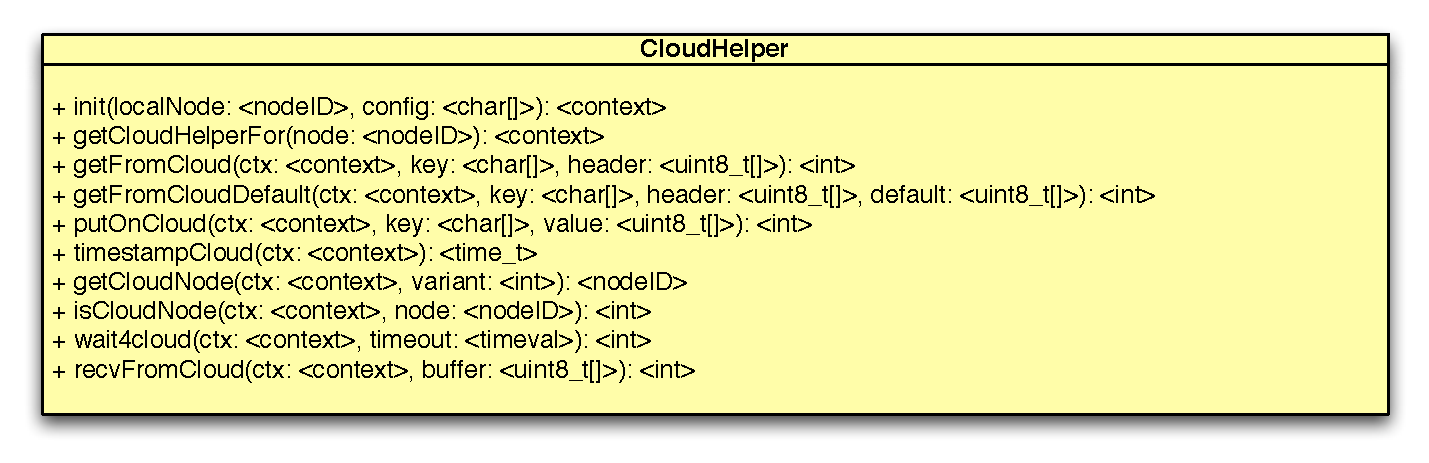
\includegraphics[width=\textwidth]{grapes-cloudhelper.pdf}
  \caption{Diagram of the \cloudhelper API.}
  \label{fig:grapes-cloudhelper}
\end{figure}

As can be seen, the functionalities offered by the API cover only the
basic storage cloud operations and the support for metadata is limited to the
last modification time: indeed at the current state only those
functions needed for the \cloudcast implementation have been
added.
Given that the purpose of the functions and their usage are for the most
part self explanatory, in the following paragraphs it is given
only a quick overview of them.
The routines \emph{get\_from\_coud()} and
\emph{get\_from\_cloud\_default()} are used to
query the cloud for a specific \emph{key}. Both of them support the
addition of custom header to the reply, to ease the processing
phase. In addition \emph{get\_from\_cloud\_default()} allows the caller to
set a default value, to be used in the event that the specified
\emph{key} is not present on the cloud. Symmetrically,
\emph{put\_on\_cloud()} takes care of updating the value of a specific
\emph{key}. All these functions use plain bytes to represent
data (in the form of array of \emph{uint8\_t}) and their return
value indicates the state of the operation: $0$ is used to signal
success, while $1$ means that an error occurred while performing the
action. The \emph{timestamp\_cloud()} function is used to obtain the time
of the last modification associated to the most recent
\emph{completed} query. A query is considered \emph{completed}
when the associated response is read. This is done via the
\emph{recv\_from\_cloud()} function, which stores the received data in the
specified buffer and returns the number of bytes read. Applications can
exploit the function \emph{wait4cloud()} to wait for the cloud to
perform a query: a return value of $1$ indicates that the
operation has been successful and the data can be read, $-1$ means that the
specified \emph{key} could not be retrieved (most likely because it is
unknown) and, finally, $0$ informs that some other error has occurred.

The two functions \emph{get\_cloud\_node()} and \emph{is\_cloud\_node()} are used
to handle the interaction with the \textit{Peer Set} module: the
former creates new peer descriptors, using the \emph{variant}
parameter to generate different instances (functionality made
necessary by implementation details of the \textit{Peer Set} module);
the latter, instead, is used to check if a specified descriptor is
indeed referring the cloud.

The remaining two functions are used to manage the execution
  context of the \cloudhelper. \textit{get\_cloud\_helper\_for()} retrieves the
\emph{context} associated to a particular peer descriptor: this
functionality is used by the \cloudcast peer sampling protocol to
fetch a configured \cloudhelper instance, without requiring
modification to the current \grapes \textit{Peer Sampling} module
API. Finally, \textit{cloud\_helper\_init()} is the function
responsible for the
creation and configuration of new \cloudhelper execution
  contexts. Adhering to the convention in use by \grapes, this function
exploits an \textit{opaque} configuration string containing a
human readable representation of the parameters.

At the current stage the only parameter directly supported by the
\cloudhelper module is represented by the string ``provider''
and it is used to select the actual implementation, which will back the
newly created \textit{context}. Such implementation will be
responsible for parsing the remaining portion of the configuration
string.

During the course of this work, two \cloudhelper implementations have been
developed. The first is backed by \textit{Amazon Simple Storage
  Service}  and it is based upon the \textit{libS3}~\cite{LibS3} library. The
second one uses a \textit{MySQL} database as storage and it
makes use of \textit{MySQL Connector/C}~\cite{MySQLConnectorC}. Both
these libraries take with them a number of dependencies and provide
synchronous operations (in contrast to the asynchronous paradigm used
by \grapes). Given the stringent restriction on dependencies and
\textit{threads} usage by the original project it has been chosen not to
include these \cloudhelper implementations directly in the code
base; instead they are available through \textit{shared libraries}.

To make this possible a \textit{fake} \cloudhelper called ``delegate''
has been developed to act as a bridge between \grapes and the \textit{shared
  libraries} implementing the actual cloud storage access. The
library name is obtained by parsing the configuration string for the parameter
``delegate\_lib''.

Figure~\ref{fig:grapes-cloudhelper-lifecycle} summarizes in a schematic
fashion this process while Table~\ref{tbl:grapes-cloudhelper-mysql}
and~\ref{tbl:grapes-cloudhelper-libs3} provide a list of the provider
specific parameters supported by the two implementations.

\begin{figure}[H]
  \centering
  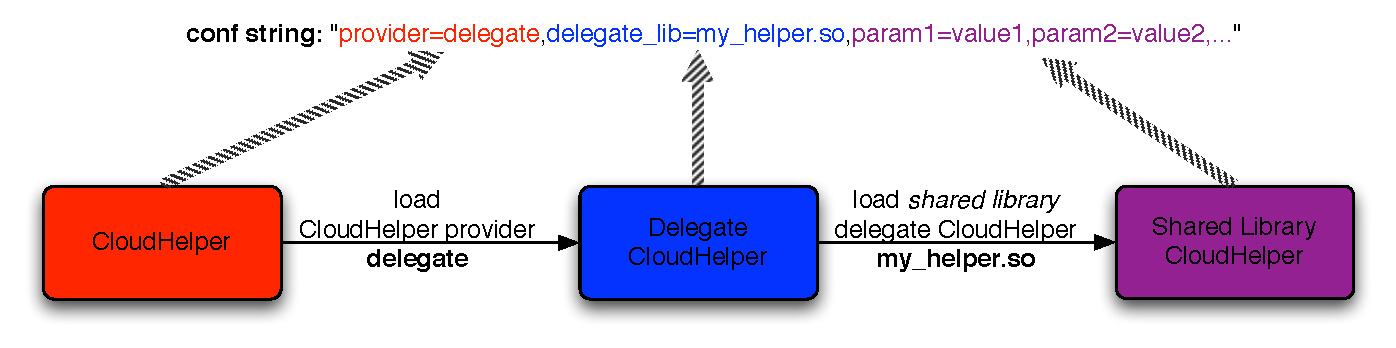
\includegraphics[width=\textwidth]{grapes-cloudhelper-lifecycle.pdf}
  \caption{\cloudhelper initialization diagram.}
  \label{fig:grapes-cloudhelper-lifecycle}
\end{figure}

\begin{table}[H]
  \centering
  \begin{tabular}{|l|l|}
  \hline
  Parameter & Meaning \\
  \hline
  \hline
  $mysql\_host$ & Hostname of the \textit{MySQL} database server \\
  $mysql\_user$ & \textit{MySQL} username \\
  $mysql\_pass$ & \textit{MySQL} password \\
  $mysql\_db$ & name of the database to use as cloud \\
  $mysql\_table$ & name of the table to use as bucket \\
  \hline
  \end{tabular}
  \caption{Provider specific parameters for \textit{MySQL} delegate helper.}
  \label{tbl:grapes-cloudhelper-mysql}
\end{table}

\begin{table}[H]
  \centering
  \begin{tabular}{|l|l|}
  \hline
  Parameter & Meaning \\
  \hline
  \hline
  $s3\_access\_key$ & \textit{Amazon} access key id \\
  $s3\_secret\_key$ & \textit{Amazon} secret access key \\
  $s3\_bucket\_name$ & name of the bucket to operate on \\
  $s3\_protocol$ & protocol used for communications. (\emph{http}  or
  \emph{https}) \\
  \hline
  \end{tabular}
  \caption{Provider specific parameters for \textit{Amazon S3} delegate helper.}
  \label{tbl:grapes-cloudhelper-libs3}
\end{table}

\section{\cloudcast peer sampling protocol}
The \cloudcast peer sampling protocol implementation is fully
integrated in the \grapes \textit{Peer Sampling} API and does not
require any specific action to be taken by the final application in
order to work. The source code follows the algorithm showed in
section~\ref{sec:cloudcast-additions} and thus is not reported
here, as it does not add any substantial contribute. Instead, this
section provides some insights on the configuration and usage of the
protocol.

Table~\ref{tbl:grapes-cloudcast-parameters} reports the supported
configuration parameters along with their meaning and default
values. As can be seen, none of them is required to obtain a fully
functional instance, however, by default, the recovery mechanism
discussed in section~\ref{sec:cloudcast-additions} is not enabled
and this may cause some problems as it is described later on.

\begin{table}[H]
  \hspace{-20pt}
  \begin{tabular}{|p{0.27\textwidth}|p{0.63\textwidth}| c |}
  \hline
  Parameter & Meaning & Default\\
  \hline
  \hline
  $period$ & period of the active cycle (\deltacyclon) in
  seconds & 10s \\
  $cache\_size$ & size of the local view ($c$) & 20 \\
  $sent\_entries$ & size of the partial view ($g$) & 5\\
  $view\_key$ & key used to host the cloud view & ``view'' \\
  $max\_silence$ & max number of global cycle without cloud
  contact (\maxsilence $*$ \deltacyclon) & 0 \\
  $cloud\_respawn\_prob$ & probability of creating a new cloud
  descriptor when silence threshold is reached (\spawnprob) defined
  in [0,1] & 0\\
  \hline
  \end{tabular}
  \caption{\cloudcast peer sampling protocol implementation
    parameters. Parenthesis enclosed values represent the
    corresponding entities in the algorithm.}
  \label{tbl:grapes-cloudcast-parameters}
\end{table}

Figure~\ref{lst:grapes-example-app} shows a minimal application which
successfully takes part in a \cloudcast peer sampling protocol
instance. The differences with respect to a standard \grapes
application which exploits the \emph{Peer Sampling} module, are limited
but substantial. First, and most notably, the \cloudhelper must be
loaded and configured. This is done in line 2 and 13-15 by including
the \textsf{cloud\_helper.h} header file and by creating a new
\textit{context}. In the example the actual cloud support is offered
by the fictional \textsf{my\_helper.so} library.
The next noteworthy operation can be seen in line 16: here the actual
peer sampling protocol is loaded by specifying the value
\textit{cloudcast} for the \textit{protocol} parameter. A custom value
is used for the \textit{cache\_size} parameter in order to give a better
understanding of the configuration mechanism.

The only remaining difference regards the handling of incoming
data. Indeed, given that \grapes design delegates the receiving of data
to the application, this is now responsible to read incoming messages
from the cloud too. To help with this task, two
commodity functions have been developed and are exposed via the
\textsf{cloud\_helper\_utils.h} header file: \textit{wait4any\_thread()} and
\textit{wait4any\_polling()}. The former concurrently invokes the wait
functions of the \textit{Network Helper} and the \cloudhelper modules,
while the second employs a polling scheme to avoid the added dependencies
that the \textit{thread} abstraction layer takes with itself. The
first variant of this functionality can be seen in action in line 25.

These are all the information needed to successfully use the
\cloudcast peer sampling protocol implemented in \grapes in a C
application. A more exhaustive documentation of the functions discussed
in this section (and many other) is provided within the headers file
distributed alongside the source code.

\begin{figure}[H]
  \centering
  \lstinputlisting[language=C,basicstyle=\footnotesize,numberstyle=\footnotesize,numbers=left,frame=leftline]{code/grapes-example.c}
  \caption{Skeleton of a simple application using the \cloudcast
    peer sampling protocol.}
  \label{lst:grapes-example-app}
\end{figure}

\section{Building and deployment}
The modifications to the toolkit have been developed with the
support of \grapes's authors and are in the process of being merged
into the main codebase. The actual code developed during the course of
this work is available via \github~\cite{GRAPES-repo}: the tag
\thesistag points to the last revision at the moment of this
writing.

The building process is unaltered and follows the conventions
established by \grapes: to generate the main library just type ``make''. This
will result in the creation of a \emph{static} library named
\textsf{libgrapes.a} containing all of the functionalities apart
for the \cloudhelper delegate implementations. These must be compiled
separately by entering in the \textsf{src/CloudSupport/} directory and
typing ``make delegate\_helpers''. Such command will build a
separate \textit{shared} library for each available delegate
helper. The \textit{PLATFORM} variable can be used to select the
desired library format: at the current state, supported values are
\textit{unix} and \textit{darwin}.
Note that before being able to compile the delegate helpers, the
\emph{libs3} and \emph{MySQL Connector/C} libraries must be
installed and configured.

\section{Java bindings}
As mentioned in the introduction, the final goal of this work is
the creation of a general framework written in \emph{Java}. This poses
the problem of how to exploit the modified \grapes toolkit from a
\emph{Java} application. In order to solve such problem, a simple
library called \jgrapes has been developed to provide the needed
bindings.

It is designed in such a way to offer a one-to-one mapping with respect
to the \grapes's modules: the available classes are
\texttt{NetworkHelper}, \texttt{CloudHelper} and
\texttt{PeerSampler}. Each one of these exposes methods mapping the
API of the respective \grapes module. The only design difference is
represented by the \texttt{JGrapes} class, which functions as a
\textit{single point of entry}: it takes care of loading the native
library and performing the required initialization action, furthermore it
provides simple functions to allocate new instances of the main
components.

The usage of the library should be evident to anyone who is already
familiar with \grapes, in any case, the package \emph{test} contains
a simple working application which shows the common usage.

Again, the library is available via \github~\cite{jGRAPES-repo}, with
the last revision at the time of this writing tagged with
\thesistag.

The building process is fully automated and makes usage of \emph{ant}
for the \emph{Java} portion and \make for the native components. The
first step is to update the \grapes distribution which will be used by
the library.
This is done by typing the command: \\
``ant update-grapes
-DGRAPES\_DIR=/path/to/grapes/distribution''.

As a result, both the
main \grapes library and the \cloudhelper delegate libraries will be
compiled and prepared to be used with \jgrapes. The same consideration
on the availability of the library dependencies made for
\grapes, applies here too. In case of errors during this phase, the
first reaction should be to check that the environment is properly
configured.

The second step is the compilation of the \emph{Java} library
itself. This is done by invoking the target \textit{dist} of the
\emph{ant} build file. During this second phase, a series of things
happens: the final \emph{shared} library is created, the \textit{Java}
toolkit is compiled and packaged and, in conclusion , all the files
required to use the functionalities are placed in the \textsf{dist/}
directory.
Since \jgrapes makes extensive use of \emph{JNI}~\cite{JNIGuide} to
complete successfully this phase, the location of \emph{JNI}'s header
files must be configured in the environment.

\section{Evaluation}
In conclusion of this chapter, we would like to show some tangible
results which demonstrate how the real implementation performs in
comparison with the simulated one.
The experiments have been performed via a \emph{Java} application
(available in the repository of \jgrapes) using the same configuration
parameters adopted by the corresponding simulations. When possible,
exactly the same settings have been employed,
but some specific experiments have been impossible to fully reproduce due to
the limited amount of time (each simulated day requires one real day)
and the lack of computational resources.

\begin{figure}[h!]
  \centering
  \subfloat[][\emph{Cloud} in-degree]{
    \hspace{-70pt}
    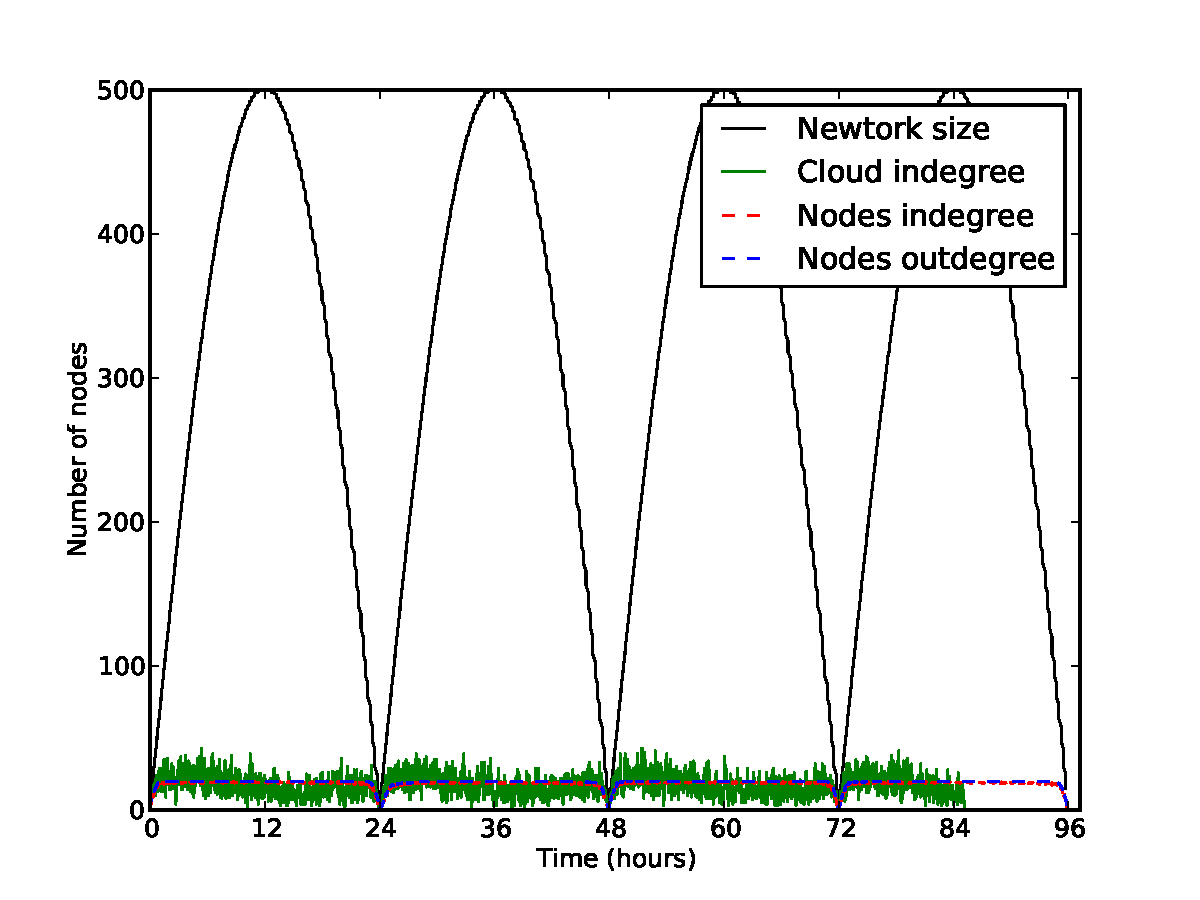
\includegraphics[width=240pt]{cloudcast-dynamic-indegree-4gg-0cloud.pdf}
    \label{fig:cloudcast-dynamic-indegree-original}
  }
  \subfloat[][\emph{Cloud} contacts]{
    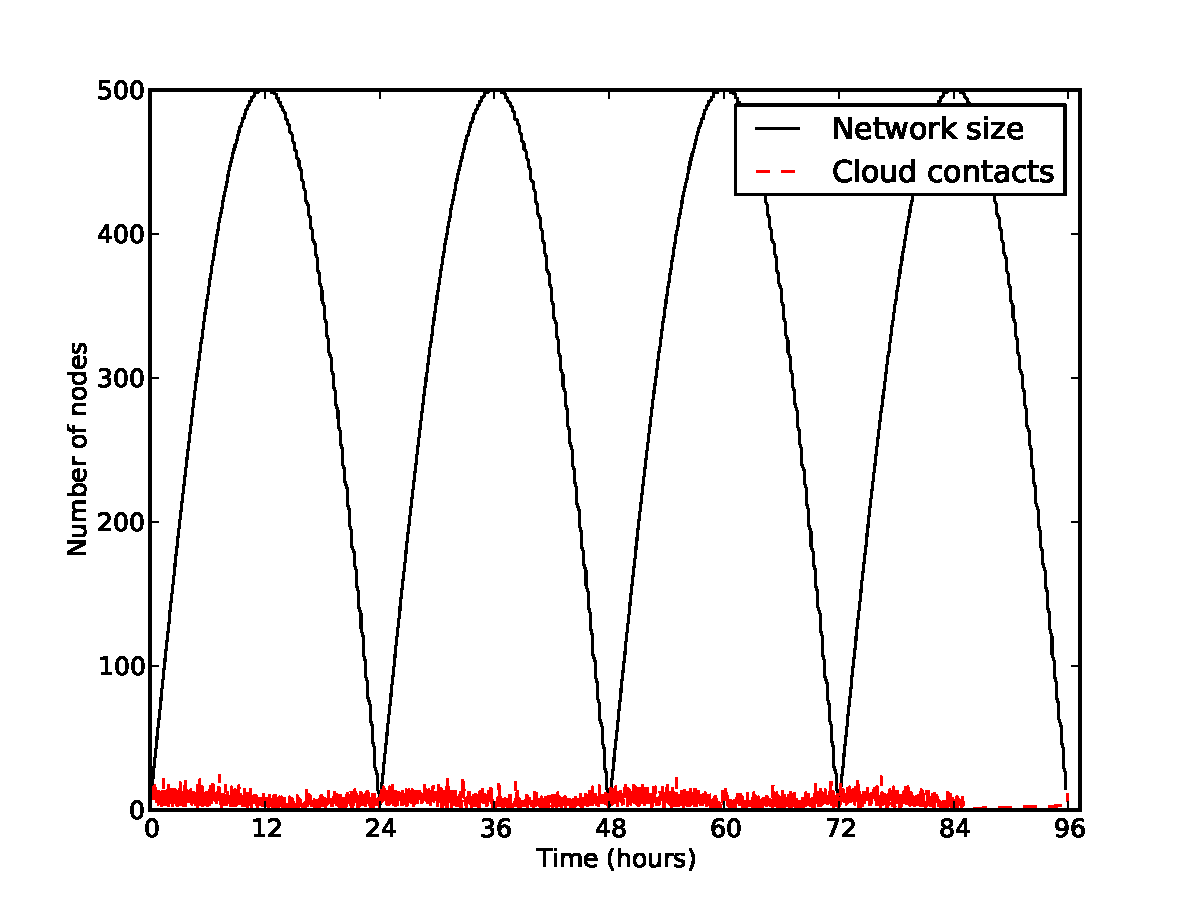
\includegraphics[width=240pt]{cloudcast-dynamic-load-4gg-0cloud.pdf}
    \label{fig:cloudcast-dynamic-load-original}
  }
  \caption{Behavior of the original peer sampling protocol}
  \label{fig:cloudcast-dynamic-original}
\end{figure}


The first result, shown in Figure~\ref{fig:cloudcast-dynamic-original}
and matching Figure~\ref{fig:cloudcast-sim-oscillating-indegree},
exhibits the behavior of the system when using the original protocol
without the recovery mechanism. As can be seen, the protocol works as
expected for the first $3$ days, maintaining the desired cloud
in-degree and contact rate, but as soon as the network starts its
descending phase on day $4$, all the cloud entries are lost and the
cloud is for all intent and purposes cut off the system. During the
analysis of \cloudcast, it has already been discussed how such a scenario
may happen, in this case, however, another factor plays an important
role. The way the \emph{Peer Set} module is currently implemented in
\grapes and the strategy used to maintain multiple cloud entries by
the modified \cyclon make so that two cloud descriptor may be
collapsed into a single one during view exchange. Such problem
requires a fairly extensive modification of the way \grapes handles
descriptors to be fixed, so it has not been feasible to correct it right
away. At any rate, on its own, the bug does not influence the behavior of
the protocol, as it is demonstrated by the first $3$ days of execution
and by extensive tests performed on fixed size networks.

\begin{figure}[h!]
  \centering
  \subfloat[][\emph{Cloud} in-degree]{
    \hspace{-70pt}
    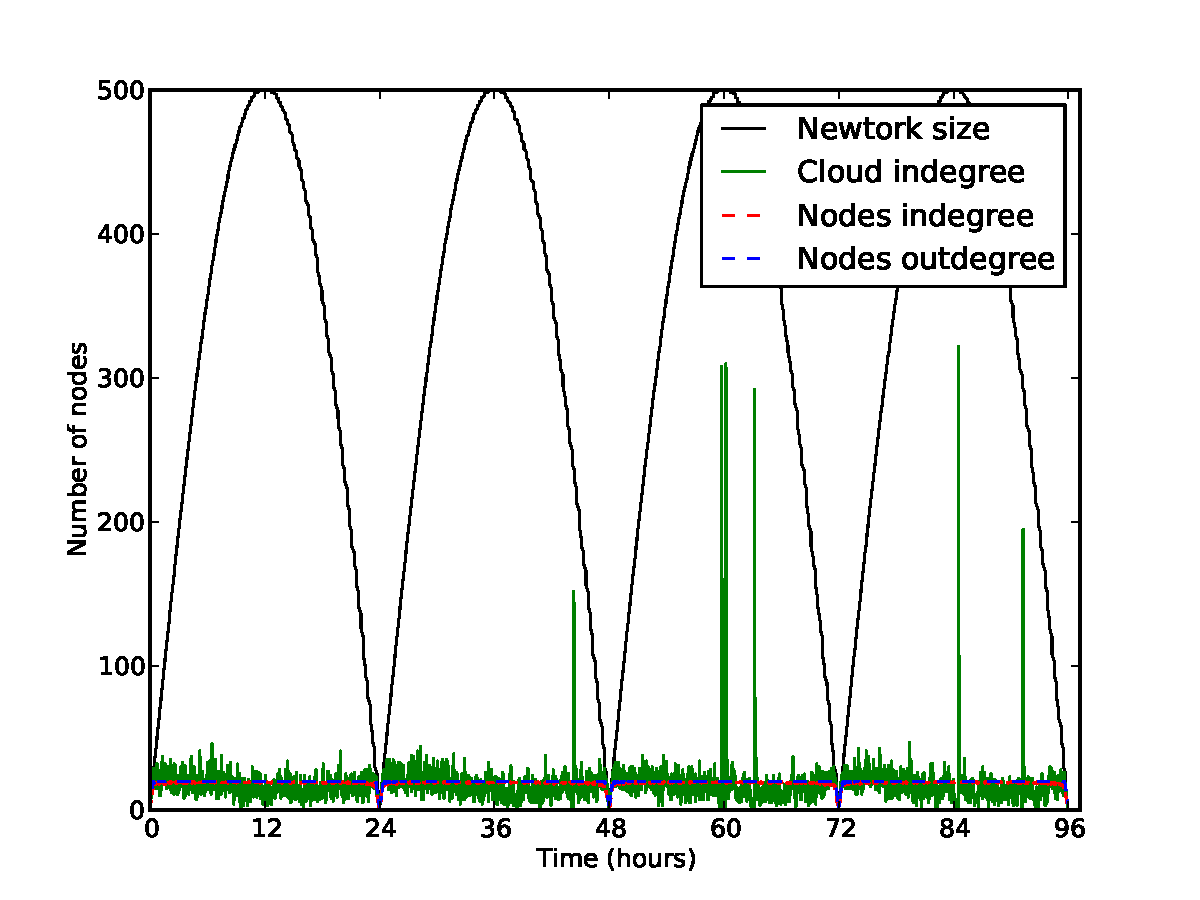
\includegraphics[width=240pt]{cloudcast-dynamic-indegree-4gg.pdf}
    \label{fig:cloudcast-dynamic-indegree-additions}
  }
  \subfloat[][\emph{Cloud} contacts]{
    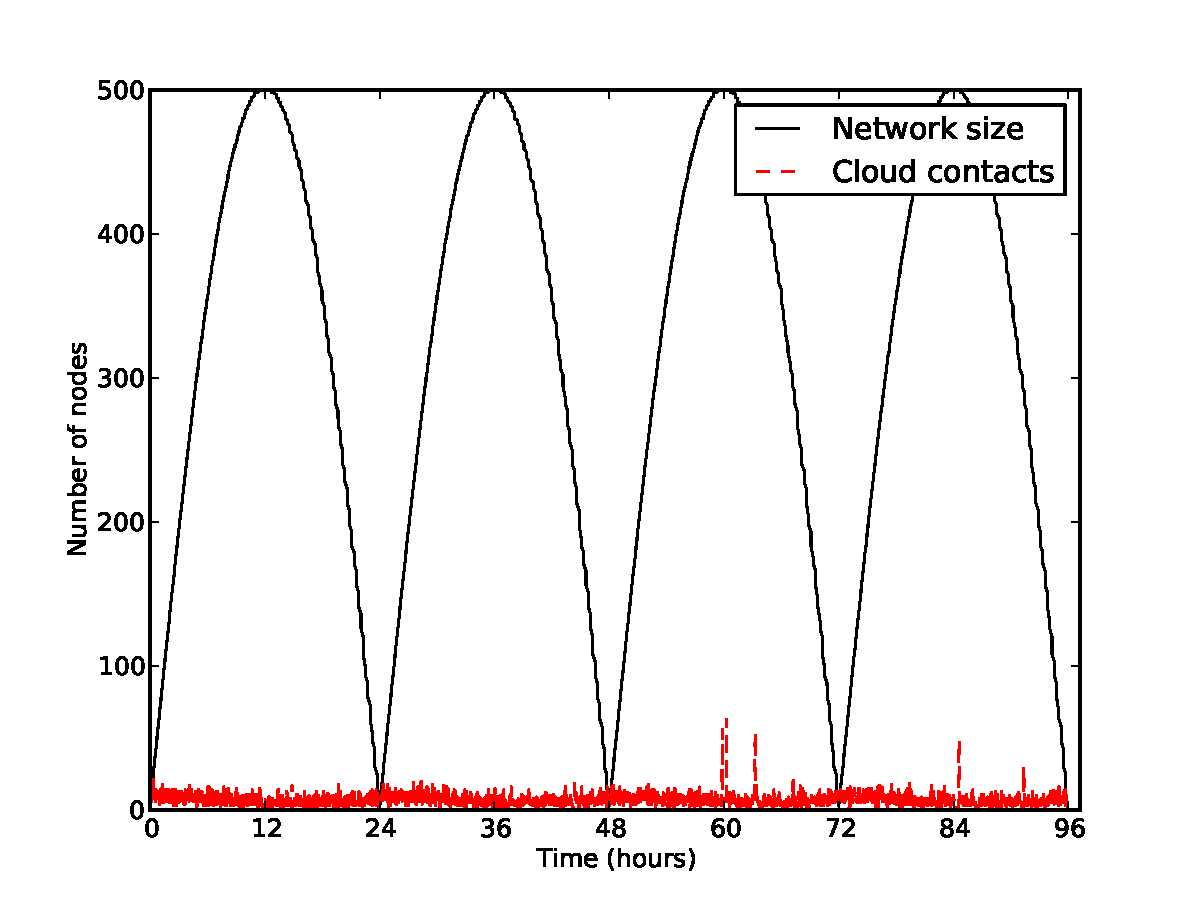
\includegraphics[width=240pt]{cloudcast-dynamic-load-4gg.pdf}
    \label{fig:cloudcast-dynamic-load-additions}
  }
  \caption{Behavior of the modified peer sampling protocol}
  \label{fig:cloudcast-dynamic-additions}
\end{figure}


Figure~\ref{fig:cloudcast-dynamic-additions} shows the same experiment
performed using the modified \cloudcast protocol. The additional
parameters used to perform these tests are:
\begin{itemize}
  \item $max\_silence$: 30 cycles
  \item $cloud\_respawn\_prob$: 0.2
\end{itemize}

The first thing that can be noted observing the
plot~\ref{fig:cloudcast-dynamic-indegree-additions} is the presence of
high peaks of cloud descriptors. This is the effect of the recovery
mechanism in action. As can be seen, the peaks are reabsorbed quickly
and, as shows plot~\ref{fig:cloudcast-dynamic-load-additions}, the
impact on the cloud contact rate is fairly limited and should not
impact much on the aggregated daily contacts.

\begin{figure}[h!]
  \centering
  \subfloat[][``clean'' run]{
    \hspace{-70pt}
    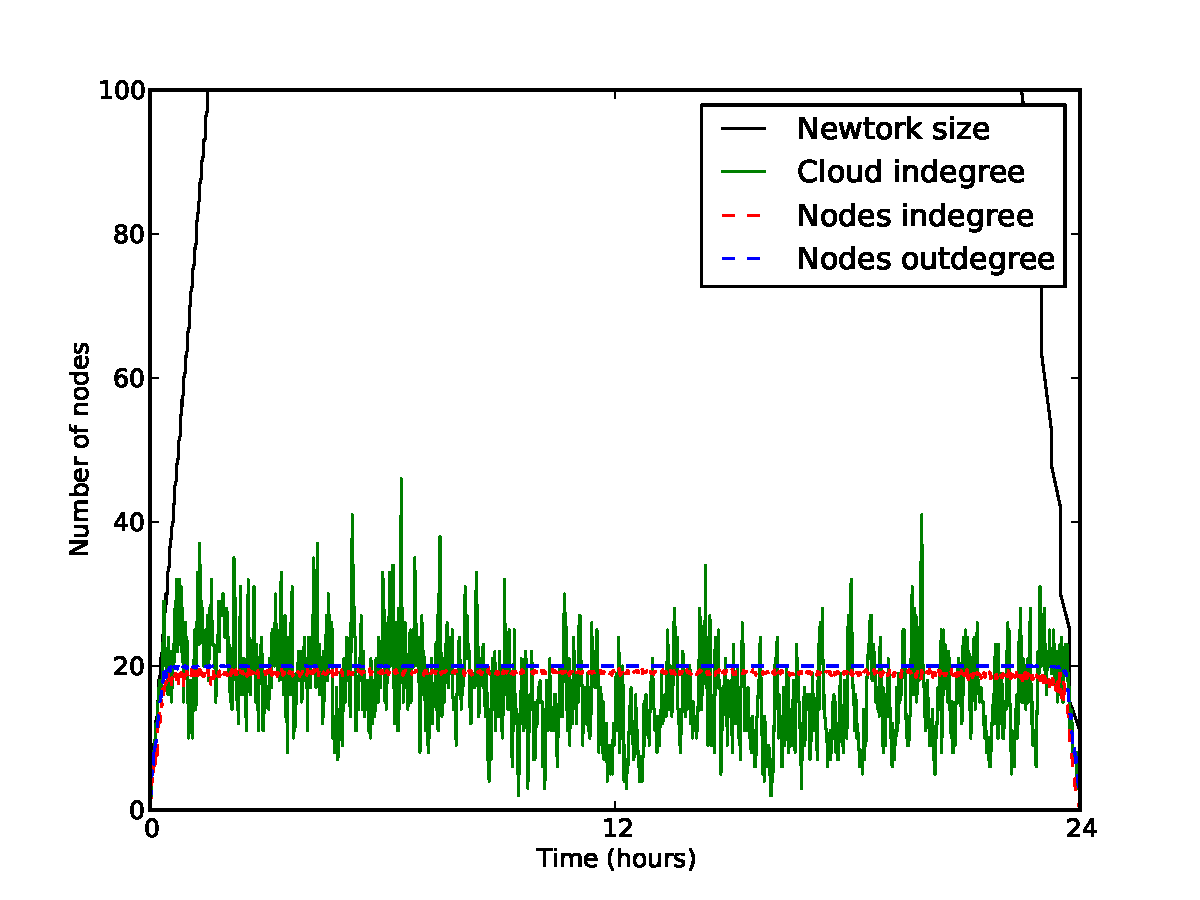
\includegraphics[width=240pt]{cloudcast-dynamic-indegree-4gg-detail-norecovery.pdf}
    \label{fig:cloudcast-dynamic-indegree-additions-detail-norecovery}
  }
  \subfloat[][Recovery mechanism in action]{
    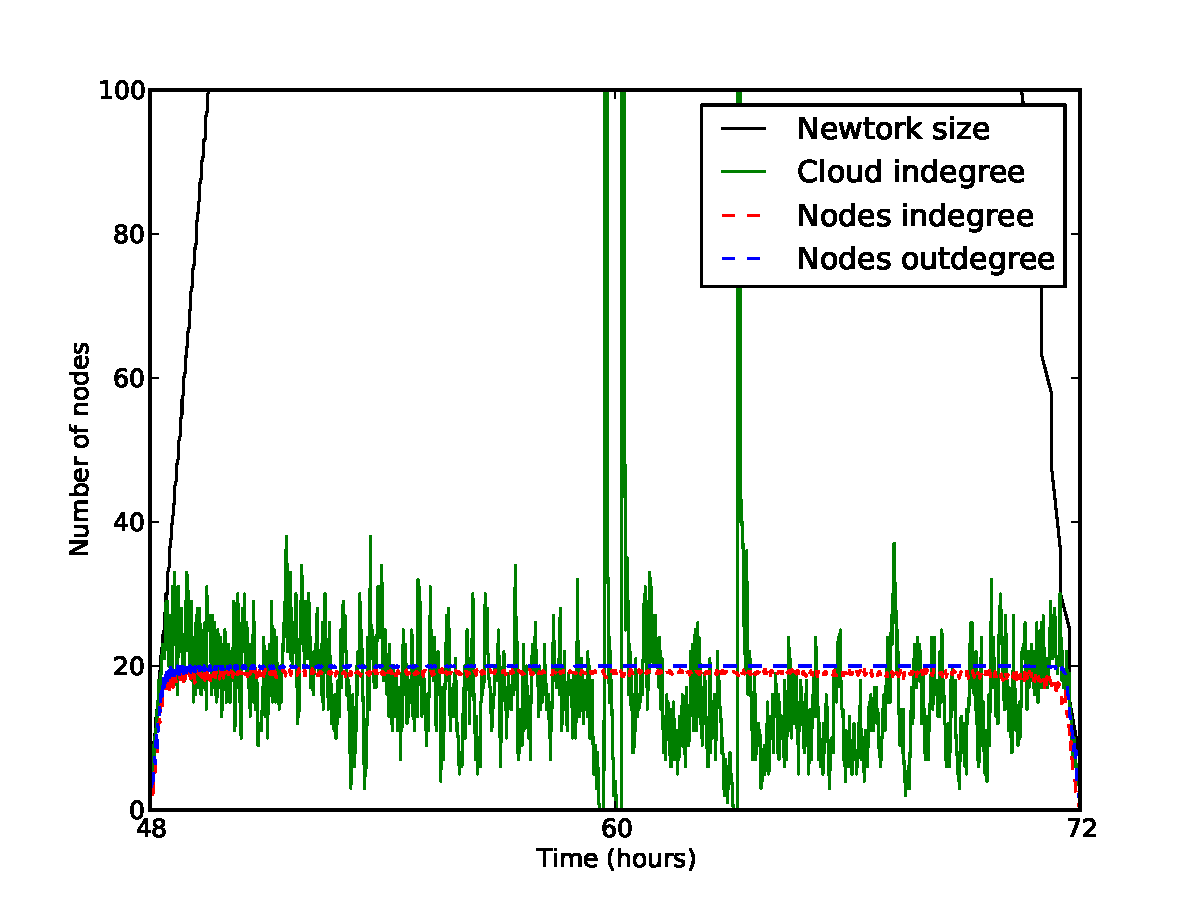
\includegraphics[width=240pt]{cloudcast-dynamic-indegree-4gg-detail-recovery.pdf}
    \label{fig:cloudcast-dynamic-indegree-additions-detail-recovery}
  }
  \caption{Zoomed-in plots comparing the effects of the recovery
    mechanism on the cloud in-degree}
  \label{fig:cloudcast-dynamic-indegree-additions-detail}
\end{figure}


Figure~\ref{fig:cloudcast-dynamic-indegree-additions-detail} shows a
comparison between a ``clean'' day of execution and another one, in which the
recovery mechanism fired multiple times. First of all, it is easy to see
how the overall performance is similar in both plots: the average
number of cloud descriptors tends, in both cases, to approximate the
desired value.
More interesting is the behavior exhibited by the recovery mechanism:
around the $60^{th}$ hour of execution it is fired 2 times in a close
succession. Such a chain of events does not happen often, but it shows
how the recovery mechanism and the cloud rate adaptive scheme work
on the two opposite fronts: the former notices that too much time has
passed since the last global cloud contact and responds by creating a
number of cloud descriptors randomly distributed in the network. The
latter reacts to the suddenly increase in contact by removing
them.
This two competing forces, alongside the usual descending phase of the
network and an unlucky succession of view exchanges, have the effect
of once more removing all the cloud entries in the network.

Considering as the starting instant the moment in which the number of
cloud descriptors goes to $0$ for the first time and as ending
instant the time in which the network stabilizes itself after the
second activation of the recovery mechanism, the total time taken by
this stalling phase is around one hour. In the meantime the protocol
still works without problems even though the target cloud contact
rate is not respected.

\begin{figure}[h!]
  \centering
  \subfloat[][``clean'' run]{
    \hspace{-70pt}
    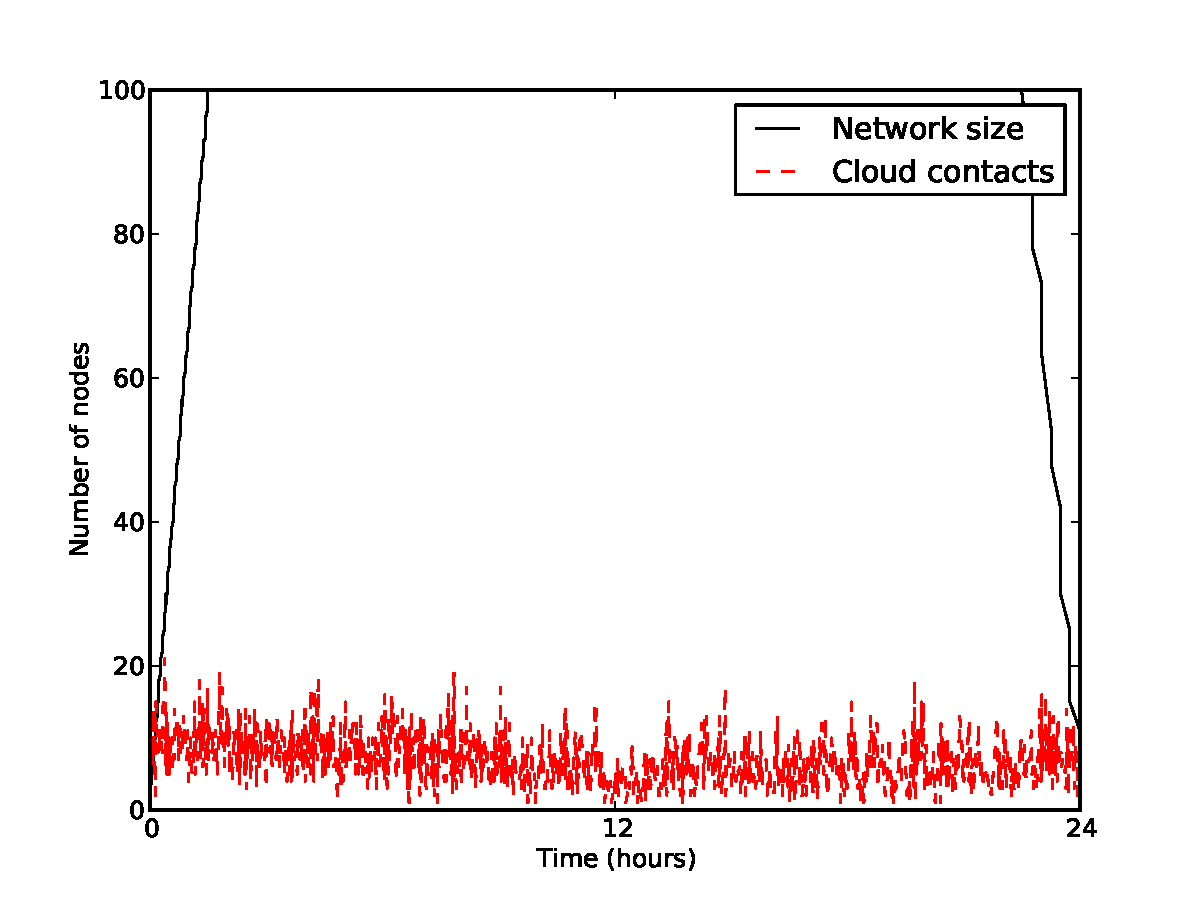
\includegraphics[width=240pt]{cloudcast-dynamic-load-4gg-detail-norecovery.pdf}
    \label{fig:cloudcast-dynamic-load-additions-detail-norecovery}
  }
  \subfloat[][Recovery mechanism in action]{
    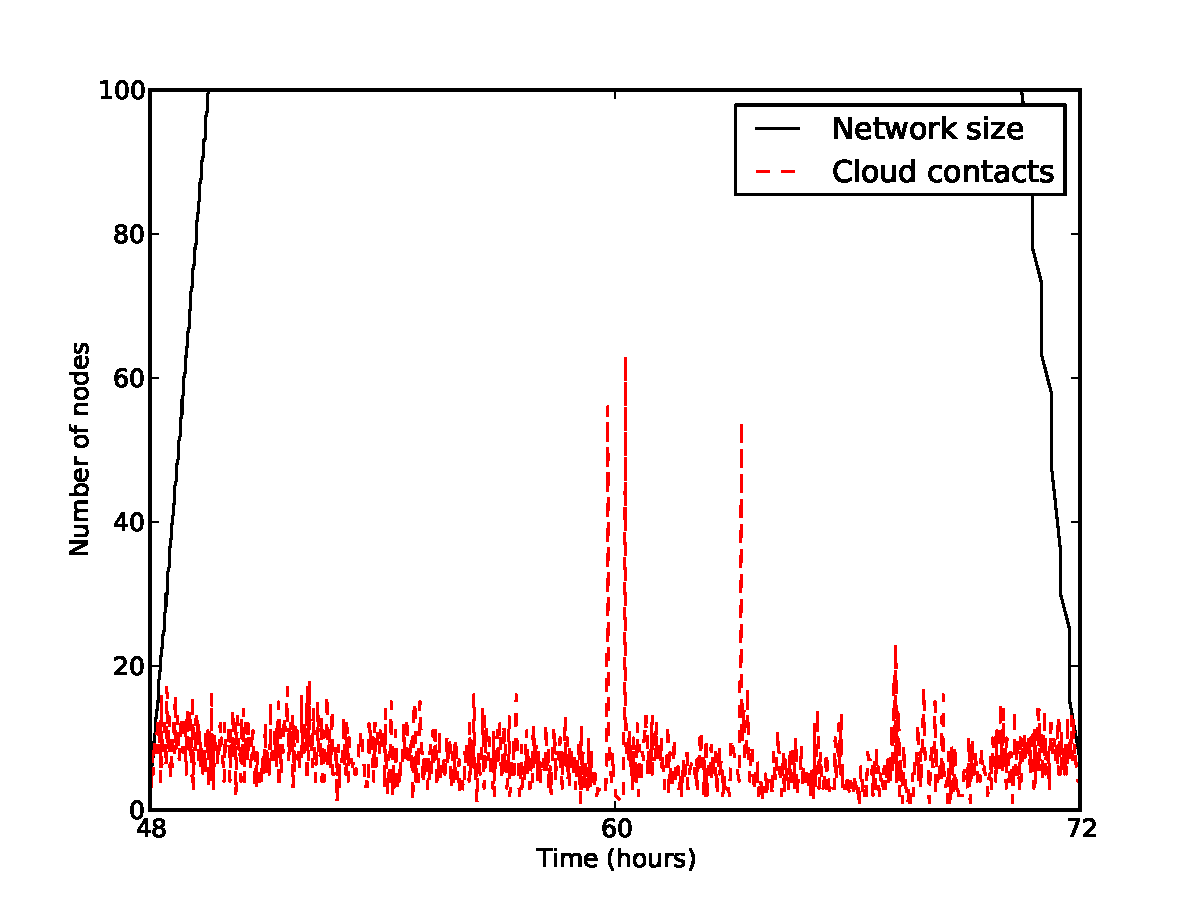
\includegraphics[width=240pt]{cloudcast-dynamic-load-4gg-detail-recovery.pdf}
    \label{fig:cloudcast-dynamic-load-additions-detail-recovery}
  }
  \caption{Detail of cloud highlighting the effects of the recovery mechanism}
  \label{fig:cloudcast-dynamic-load-additions-detail}
\end{figure}

Figure~\ref{fig:cloudcast-dynamic-load-additions-detail} shows the
same two days from the point of view of the cloud contact rate. In
these plots is more evident how limited is the influence of the
recovery mechanism: the peaks are relatively small and they last for a
limited amount of time.

The parameters used to configure the recovery mechanism have not been
subjected to evaluation; they have been selected so to be somewhat
realistic but without any deep consideration on their impact. Thus,
by selecting them more carefully or even better by employing some
adaptive strategy, the imposed overhead should sensibly decrease.

\begin{figure}[h!]
  \centering
  \subfloat[][Real implementation results]{
    \hspace{-70pt}
    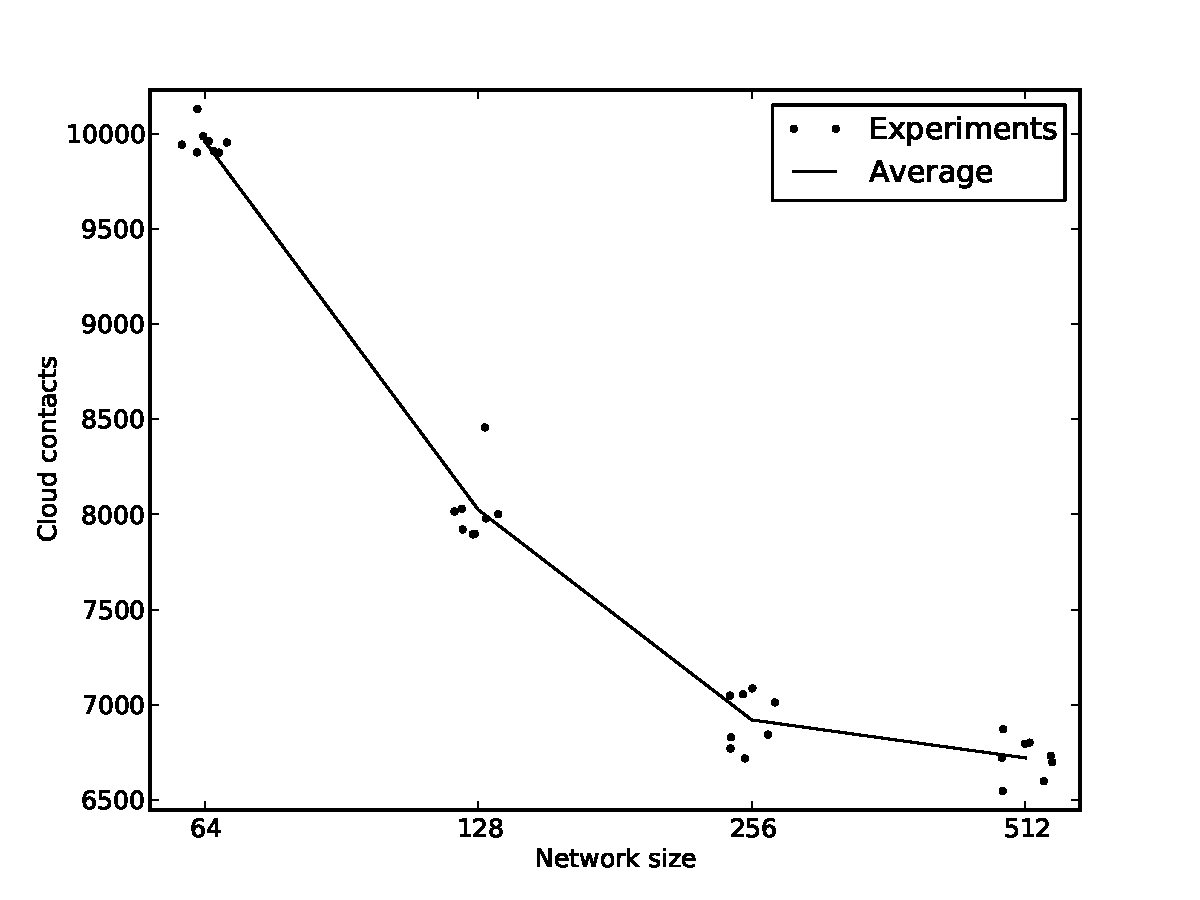
\includegraphics[width=240pt]{cloudcast-loads.pdf}
    \label{fig:cloudcast-loads}
  }
  \subfloat[][Simulated results]{
    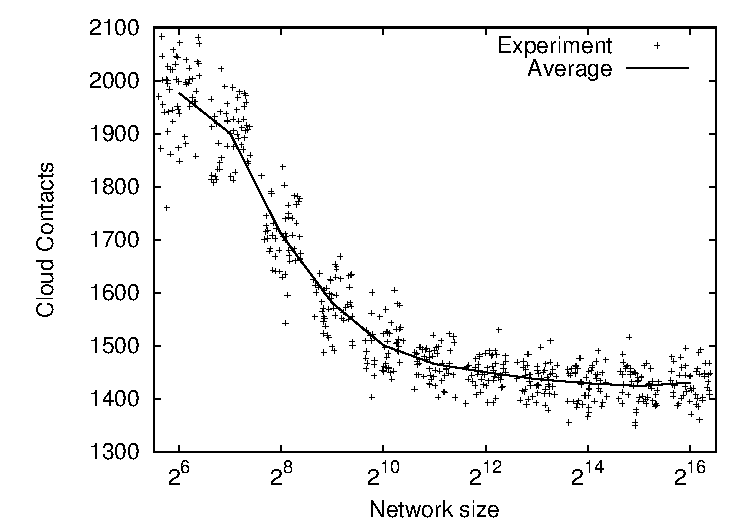
\includegraphics[width=240pt]{cloudcast-sim-loads.pdf}
    \label{fig:cloudcast-sim-loads-re}
  }
  \caption{Storage cloud load for different network sizes.}
  \label{fig:cloudcast-loads-global}
\end{figure}

Figure~\ref{fig:cloudcast-loads-global} concludes the evaluation of the
work performed on \grapes. The plot~\ref{fig:cloudcast-loads} shows the cloud
load obtained by the implementation for different network
sizes and matches the plot in Figure~\ref{fig:cloudcast-sim-loads} which
is repeated here for convenience.

Due to differences in the experiment setup and in the way data has been
collected, the values in the two plots are not directly comparable,
however it is evident how they are proportional. In both cases the cloud
contact rate is high for small networks and it tends to decrease as
more nodes are added.

Denser networks have not been tested, since the shared servers at our
disposal were not able to sustain the high computation load caused by
the extensive use of Java threads.
